\begin{figure}[tbp]
\centering
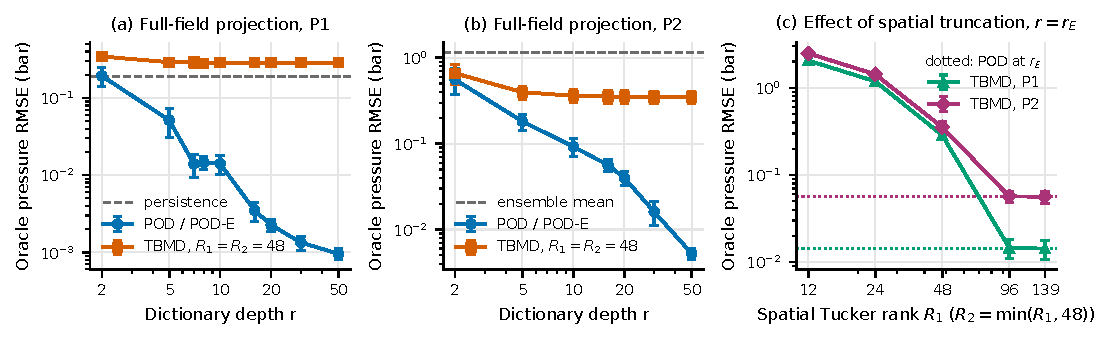
\includegraphics[width=\textwidth]{../../../../studies/brugge_sparse_sensing/figures/fig3_representation.pdf}
\caption{Representation capacity with all active channels observed (least-squares projection of held-out snapshots). (a, b) Pressure RMSE against dictionary depth $r$ for POD/POD-E (identical subspace) and TBMD with spatial ranks $(48,48,2)$ in P1 and P2; dashed line: no-measurement reference. (c) TBMD pressure RMSE against the spatial Tucker rank $R_1$ ($R_2=\min(R_1,48)$, $R_3=2$) at the training-selected depth; dotted lines: POD at the same depth. Markers: mean over ten folds; bars: one standard deviation.}
\label{fig:representation}
\end{figure}
